%% 1.tex

\textbf{Exercise 1.} \emph{A Poisson process with rate \( \lambda > 0 \) can be defined as a counting process \( \{N(t):\, t \geq 0\} \) with the following properties:}
\begin{enumerate}
  \item[\textit{(i)}] \emph{\( N(0) = 0 \)}.
  \item[\textit{(ii)}] \( N(t) \) \emph{has independent and stationary increments}.
  \item[\textit{(iii)}] \emph{Let \( \Delta N(t)  = N(t + \Delta t) - N(t)\) with $\Delta t > 0$. The following relations hold: }
        \[
        \begin{aligned}
          P[\Delta N(t) = 0] &= 1 - \lambda \Delta t + o(\Delta t),\\
          P[\Delta N(t) = 1] &= \lambda \Delta t + o(\Delta t),\\
          P[\Delta N(t) \geq 2] &= o(\Delta t).\\
        \end{aligned}
        \]
\end{enumerate}
\emph{From this definition show that}
\begin{equation}\label{eq:1}
  P[N(t) = n] = \frac{1}{n!}\lambda^{n}t^{n} e^{-\lambda t}.
\end{equation}

\emph{To this end, set up a system of differential equations for the quantities \( P[N(t) = 0] \) and \( P[N(t) = n] \) with \( n \geq 1 \). Then verify that Eq.~\eqref{eq:1} satisfies the differential equations derived.}

\emph{Illustrate the validity of the derivation by comparing the empirical distribution obtained in a simulation of the Poisson process and the theoretical distribution of \( P[N(t) = n ]\) given by Eq.~\eqref{eq:1} for the values \( \lambda = 10 \) and \( t = 2 \).}

\emph{Solution. }We begin by deriving the differential equation for \( P[N(t) = 0]\). Given $\Delta t > 0$, we have:
\[
  \begin{aligned}
    P[N(t + \Delta t) = 0] &\stackrel{(ii)}{=} P[N(t) = 0]P[\Delta N(t) = 0]\\
    &\stackrel{(iii)}{=} P[N(t) = 0](1- \lambda\Delta t + o(\Delta t))\\
    &= P[N(t) = 0] - P[N(t) = 0]\lambda\Delta t + o(\Delta t).
    \end{aligned}
  \]
  Rearranging and dividing both sides by \( \Delta t \), we get
  \[
    \frac{P[N(t + \Delta t) = 0] - P[N(t) = 0]}{\Delta t} = - \lambda P[N(t) = 0] + \frac{o(\Delta t)}{\Delta t}.
  \]
  Finally, we obtain the desired differential equation by letting $\Delta t \to 0^+$:
\[
  \frac{d}{dt}P[N(t) = 0] = -\lambda P[N(t) = 0],
\]
where the last term vanishes by definition of \( o(\cdot) \):
  \[
    \lim_{\Delta t \to 0^{+}}\frac{o(\Delta t)}{\Delta t} = 0.
  \]
It is well-known that the solution to this differential equation with initial condition \( P[N(0) = 0] = 1 \) is
\[
  P[N(t) = 0] = e^{-\lambda t}.
\]
We can now tackle the general case. Firstly, for a fixed \( n \geq 1 \) we notice that the event \(  N(t + \Delta t) = n \) can happen in three different ways:
\begin{enumerate}
  \item There are no events between times $t$ and \( \Delta t \): \(  N(t) = n \) and \(\Delta N(t) = 0\).
  \item There is one event between $t$ and \( \Delta t \): \(N(t) = n-1\) and \(\Delta N(t) = 1 \).
\item There is more than one event between $t$ and \( \Delta t \): \(  N(t + \Delta t) = n \) and \(\Delta N(t)  \geq 2\).
\end{enumerate}
Thus, since the increments are independent, we have
\begin{equation}
  \label{eq:desc}
  \begin{aligned}
    P[N(t + \Delta t) = n] &= P[N(t) = n]P[\Delta N(t) = 0]\\
    &\ + P[N(t) = n-1]P[\Delta N(t) = 1] \\
    &\ + P[N(t+\Delta t)=n \mid \Delta N(t)\geq 2]P[\Delta N(t)\geq 2].\\
    \end{aligned}
  \end{equation}
  We can expand the expressions in which $\Delta N(t)$ is involved by virtue of $(iii)$, noting that some terms will be negligible when divided by $\Delta t \to 0^+$. In particular, since the last term in the RHS of Eq. \eqref{eq:desc} is smaller than $P[\Delta N(t)\geq 2]$ and the latter is $o(\Delta t)$, the former is $o(\Delta t)$ as a whole. Following the same reasoning as before, we have:
  \[
    \frac{P[N(t + \Delta t) = n] - P[N(t) = n]}{\Delta t} = -\lambda P[N(t) = n] + \lambda P[N(t) = n-1] + \frac{o(\Delta t)}{\Delta t}.
  \]
  Letting \( \Delta t \to 0^{+} \), we get:
  \[
    \frac{d}{dt}P[N(t) = n] =  -\lambda P[N(t) = n] + \lambda P[N(t) = n-1].
  \]
  Rearranging and multiplying both sided by \( e^{\lambda t} \) yields:
\[
  e^{\lambda t}\left( \frac{d}{dt}P[N(t) = n] + \lambda P[N(t) = n] \right) = e^{\lambda t}\lambda P[N(t) = n-1].
\]
Now we realize that the left hand side is the result of applying Leibniz's product differentiation rule to a certain pair of functions. Indeed, it is easy to see that the above expression is equivalent to:
\begin{equation}
  \label{eq:difeq}
  \frac{d}{dt} \left(e^{\lambda t}P[N(t) = n] \right)= e^{\lambda t}\lambda P[N(t) = n-1].
\end{equation}

We will find a closed-form solution to Eq. \eqref{eq:difeq} via induction. For $n=1$, since we already know that \( P[N(t) = 0] = e^{-\lambda t}  \), we have:
\[
   \frac{d}{dt} e^{\lambda t}P[N(t) = 1] = e^{\lambda t}\lambda P[N(t) = 0] = \lambda e^{-\lambda t}e^{\lambda t} = \lambda.
 \]

Integrating in both sides w.r.t $t$, we arrive at
\[
e^{\lambda t}P[N(t)=1] = \lambda t + C \implies P[N(t)=1] = \lambda t e^{-\lambda t} + e^{-\lambda t}C,
\]
but $C$ must be zero to fulfill the initial condition $P[N(0)=1]=0$. Next, we assume that the solution for $n-1$ is:
\[
P[N(t) = n-1] = \frac{1}{(n-1)!}\lambda^{n-1}t^{n-1} e^{-\lambda t},
\]
and we will prove the desired equality for $n$. Applying the induction hypothesis, we have:
 \[
    \frac{d}{dt} e^{\lambda t}P[N(t) = n] = e^{\lambda t}\lambda P[N(t) = n-1] = \frac{1}{(n-1)!}\lambda^{n}t^{n-1}.
 \]
Integrating in both sides yields
\[
  e^{\lambda t}P[N(t) = n] = \frac{1}{n!}\lambda^{n}t^{n} + C \implies P[N(t) = n] = \frac{1}{n!}\lambda^{n}t^{n}e^{-\lambda t} + e^{-\lambda t}C,
\]
but again \( C = 0 \) since \( P[N(0) = n] = 0\). Thus the inductive step is completed, and the proof is concluded.

\hfill $\square$

To illustrate the result, we compare the theoretical distribution given by Eq \eqref{eq:1}} (which is a Poisson distribution with parameter $\lambda t$) and the result of many simulations of a Poisson process. In particular, we use two strategies for simulating such a process: one that leverages the fact that interarrival times follow an exponential distribution; and one that uses the order statistics of a certain uniform distribution (see Exercise 3).

Below are the results for 1000 independent simulations with a fixed value of $\lambda = 10$ and $t=2$. That is, we are interested in counting the number of events up to the time instant $t=2$ in a Poisson process governed by a rate $\lambda=10$.

\begin{figure}[h!]
  \centering
  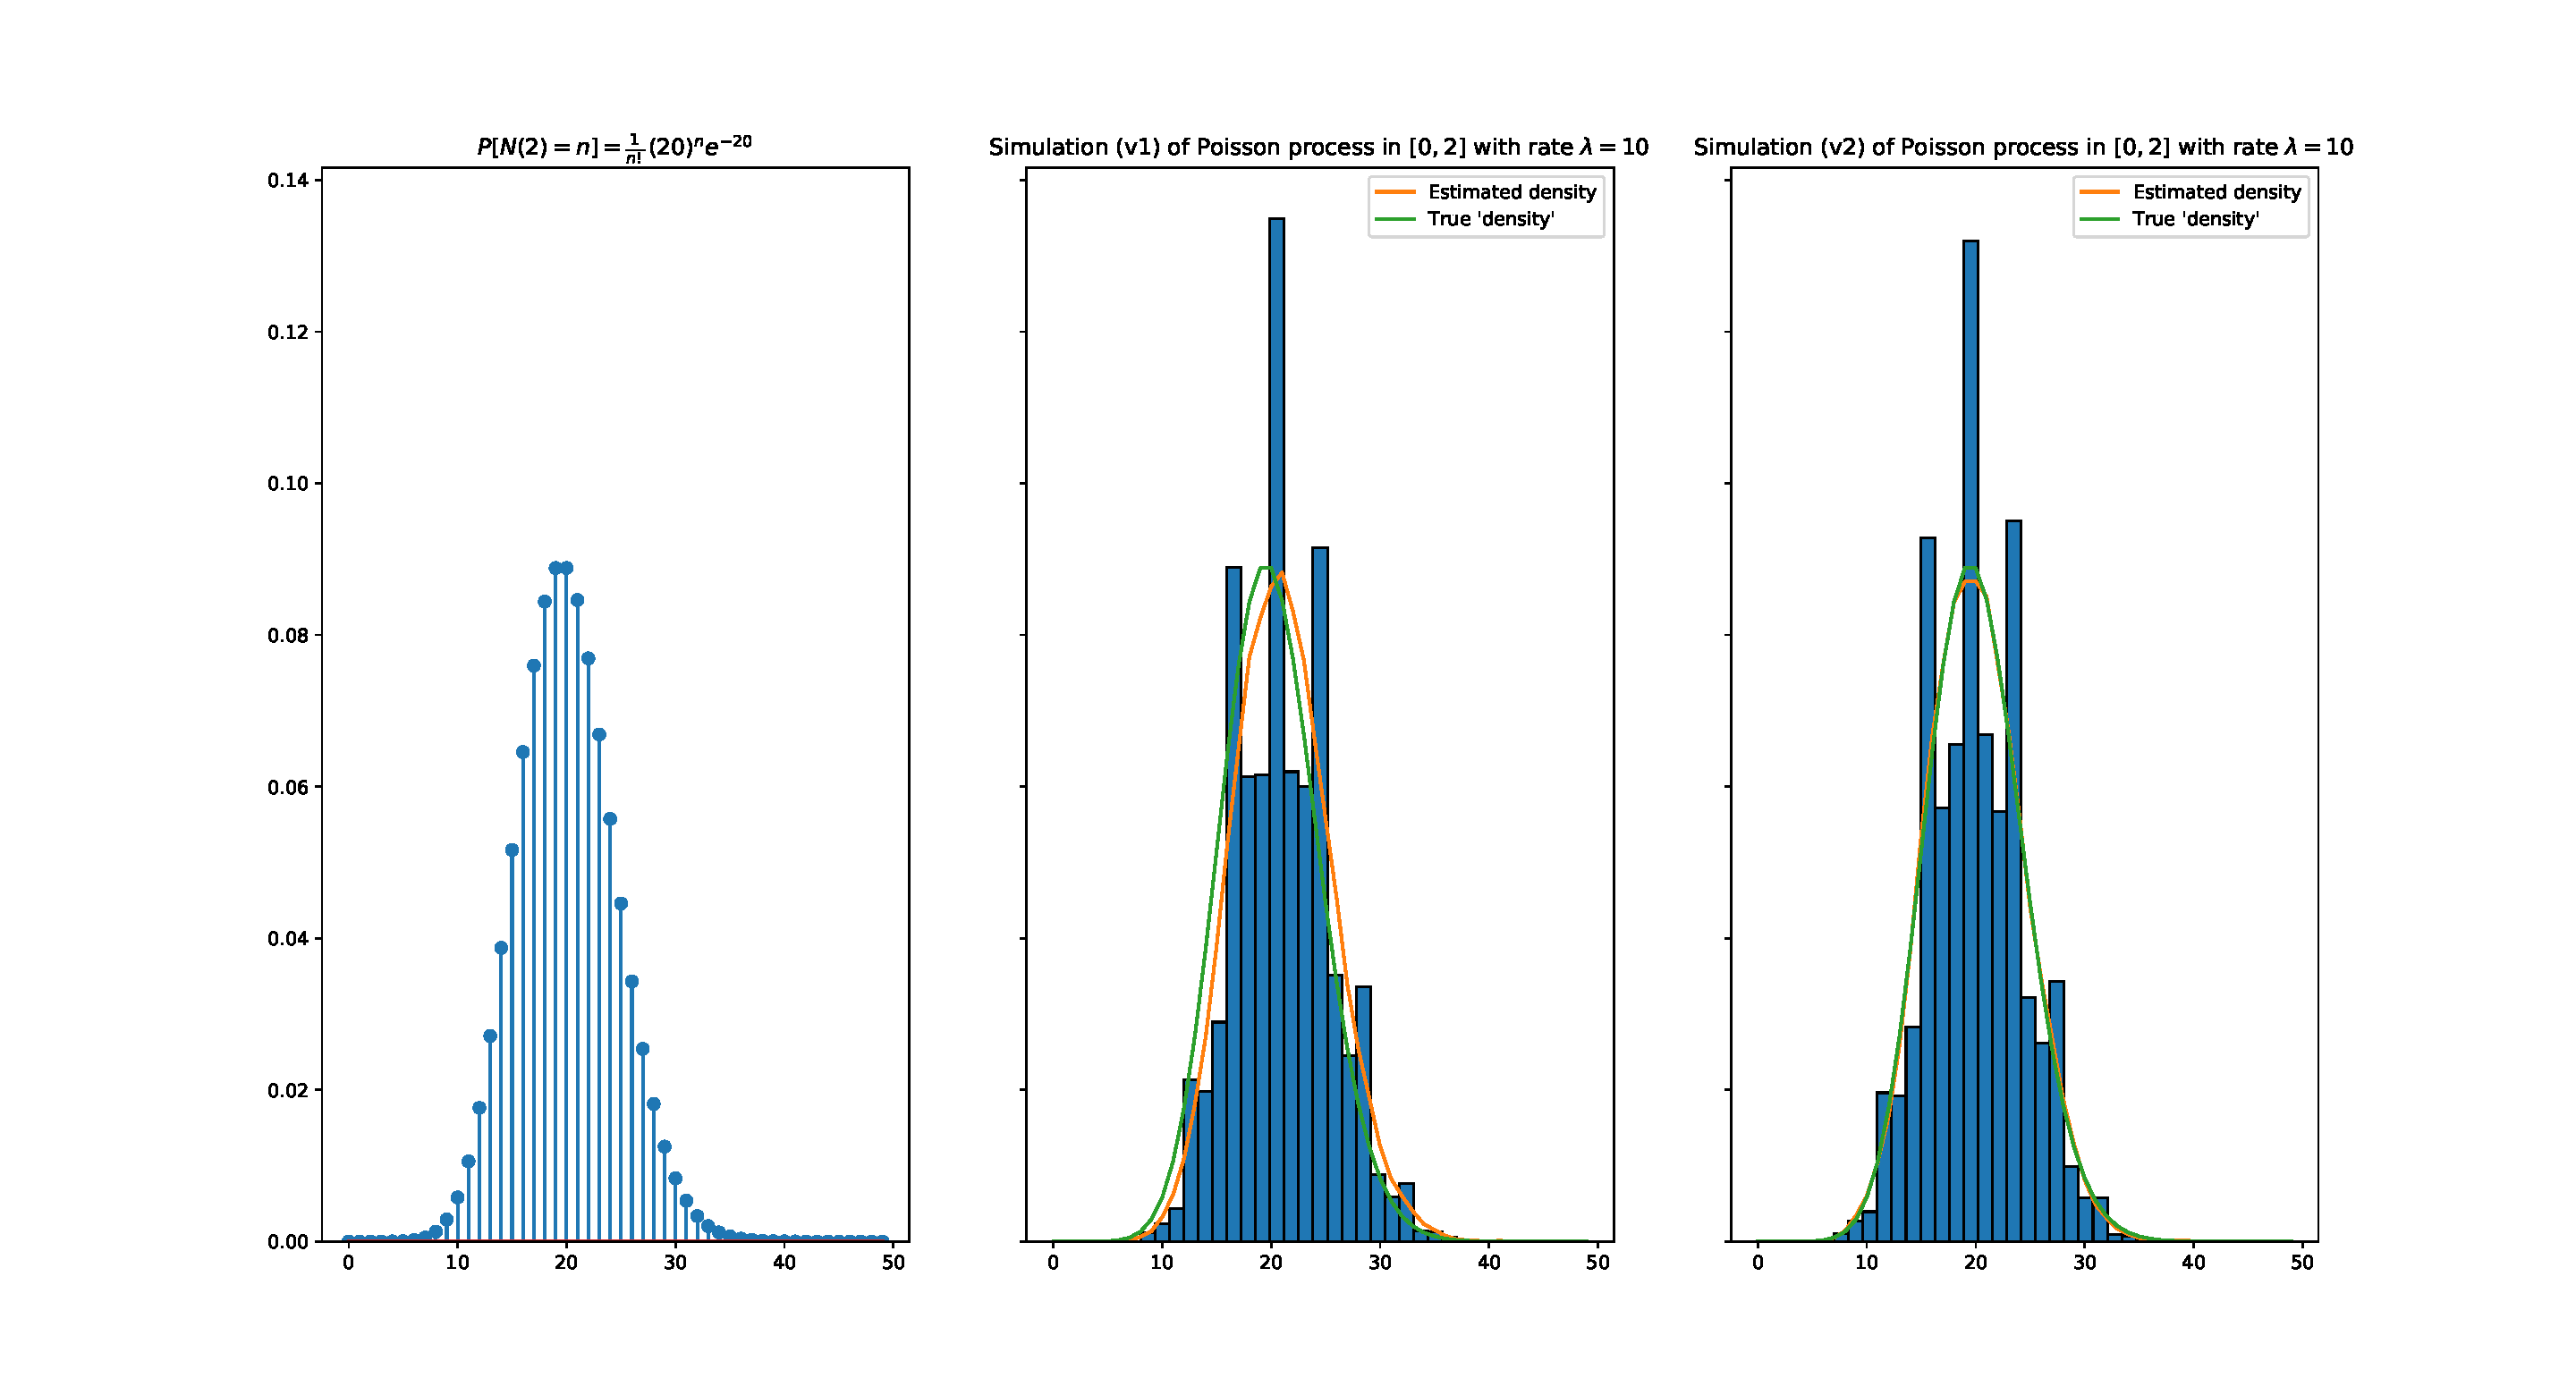
\includegraphics[width=\textwidth]{img/ex1.pdf}
\end{figure}

The leftmost graph shows the theoretical distribution, and the other two are the result of the simulations with each strategy. We also superimpose the estimated kernel density (via a Gausian kernel) and the ``true'' density, that is, the theoretical pmf of the Poisson distribution in which the points have been joined in a continuous line. We can see that the simulations accurately represent the theoretical distribution.
